We hypothesize that with the gamification of a complex combinatorial problem in architectural design provides a user an innovative means to improve their design and gradually reach optimality. We also hypothesize that competitive co-design is an effective solution to the non-convex optimization problem that is crowd-aware environment design for efficient evacuation. We have conducted some user studies below to evaluate our hypothesis.

\subsection{User Study}
For our first hypothesis, we evaluated the evacuation times of certain user iterations for each of the 54 combinations of crowd configuration parameters. We have considered only the data of an user who has viewed the heat map for every iteration. For the second hypothesis, for each of the game level and each of the crowd parameter combination we have plotted all the evacuation times of user simulation runs in order of time of execution. We have considered the data of the users who have viewed the best scorer's heat map. 

Each player is identified by a unique id assigned to him/her. Some of the user data we gathered are Player id, User placed architectural element positions, Total evacuation time of the simulation, User choices of crowd configuration parameters (LoS, LoA, LoH), User's choice of viewing the heat map, User's choice of viewing the Top Scorer's heat map. 

\subsubsection{Procedure}
We have provided the user an existing layout at the start of the level which helps us increase the difficulty as the user gradually reaches higher levels. Users cannot manipulate these already placed elements. Users can create a wall by clicking on two points in the layout. Pillars can be created by clicking at a point, on the floor, where the player want to place the pillar. The radius of the pillar can be changed by playing around with the slider in the creation menu. Doors can be created by clicking on the walls where the user wants to place the door. Walls, doors and pillars created by the user can be deleted by selecting them again. There are keyboard keys assigned to increase or decrease the width of the wall to be placed. Walls can be moved around by clicking them and using the arrows keys or by dragging them with the use of a mouse.

There are several constraints associated with each element in the layout. First of all the users cannot modify the elements of the layout existing when the level started. Users can only manipulate the elements they added to the existing layout. There are a fixed number of walls, pillars and doors that can be placed by the user.  Walls can be placed only if it forms an enclosed space meaning that a wall must be touching walls on either end. A wall cannot be made to pass through the outside wall. In case the wall is placed incorrectly by the player, the wall will be marked red, and the player will not be able to start the simulation until the errors are rectified. If the width of the wall is less than two units, the wall will not be created.

\begin{figure*}[ht] 
\centering
\begin{tabular}{c c c c c}
	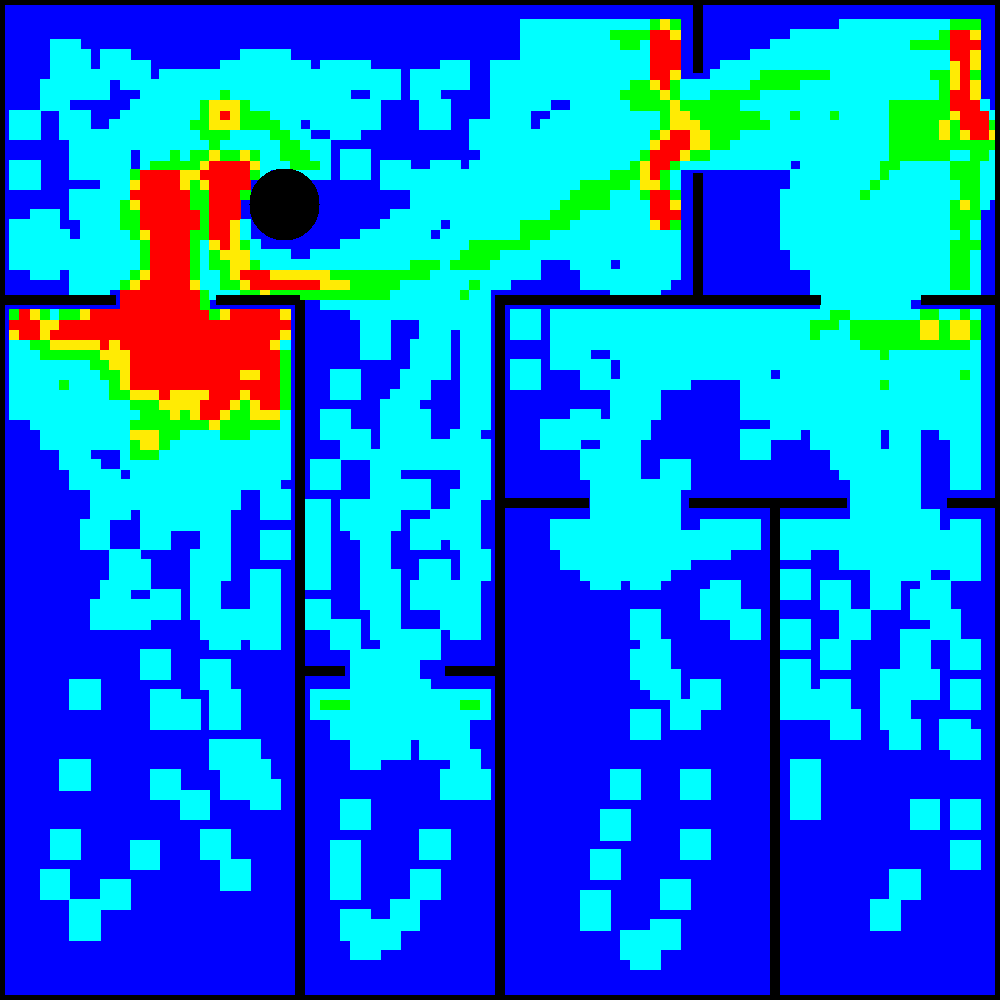
\includegraphics[width=0.19\textwidth]{images/Hypothesis2/Iter1-ID-12_t_16_4175.png} & 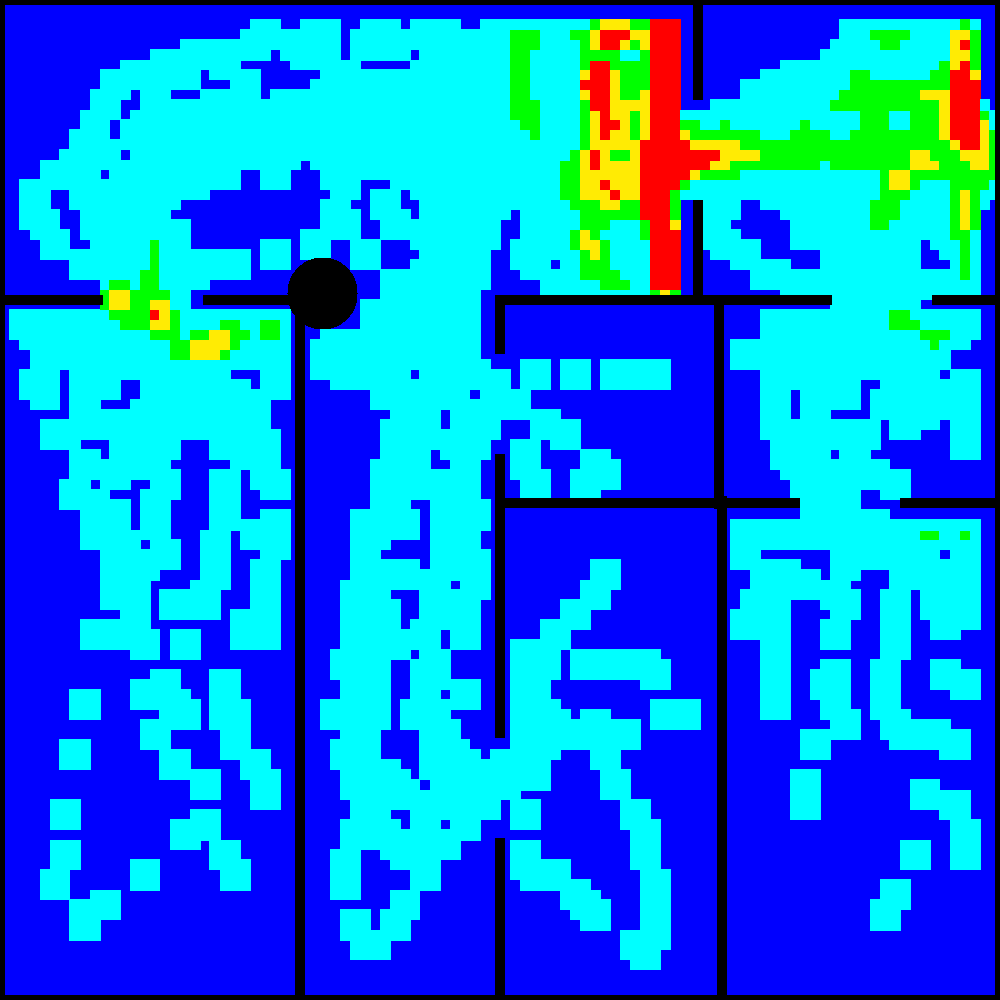
\includegraphics[width=0.19\textwidth]{images/Hypothesis2/Iter2-ID-8_t_13_695.png} & 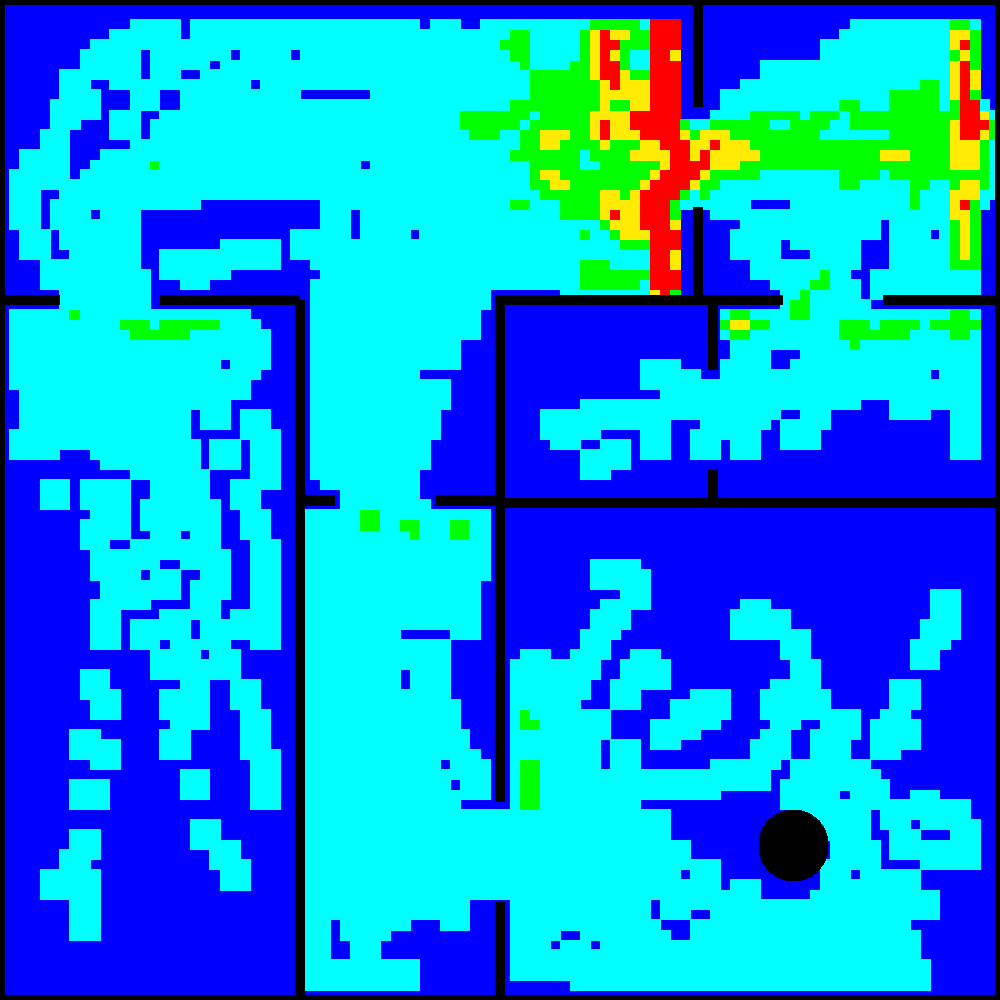
\includegraphics[width=0.19\textwidth]{images/Hypothesis2/Iter3-ID-22-t_11_1705.png} & 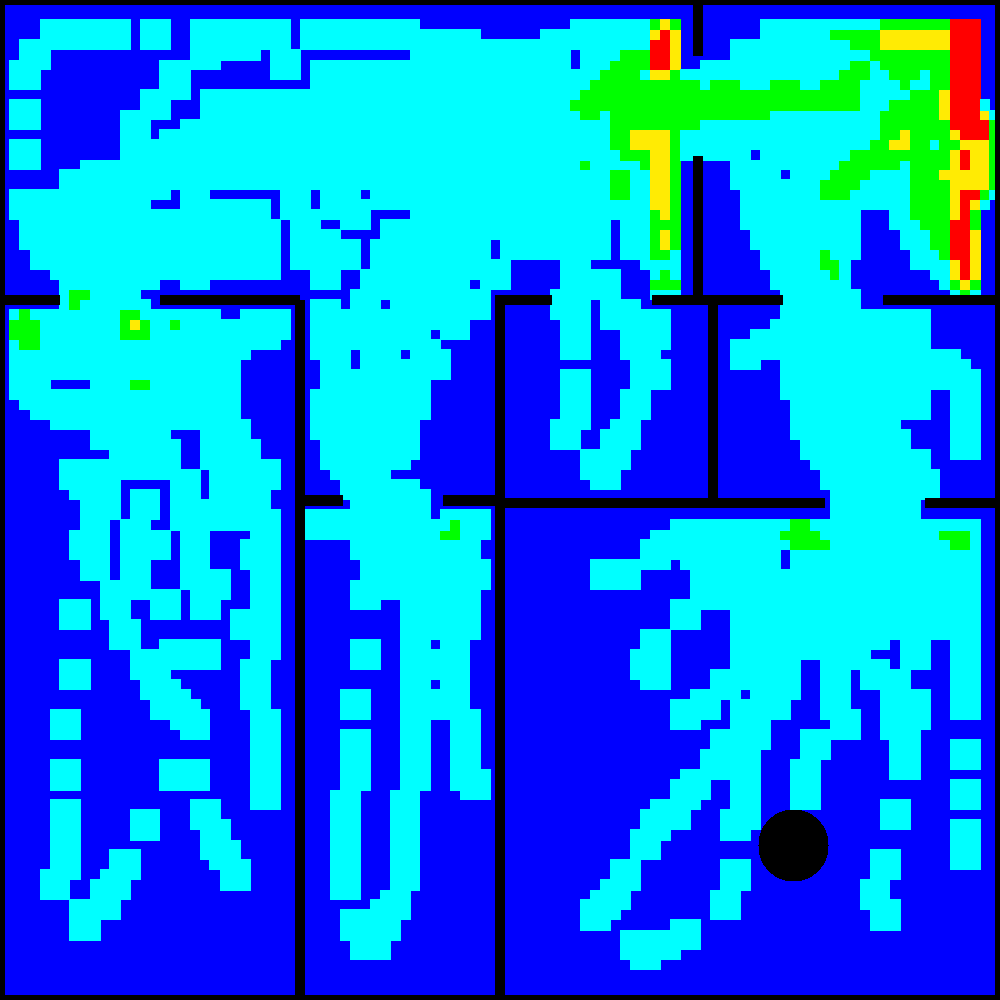
\includegraphics[width=0.19\textwidth]{images/Hypothesis2/Iter4-ID-17-t_9_669.png} & 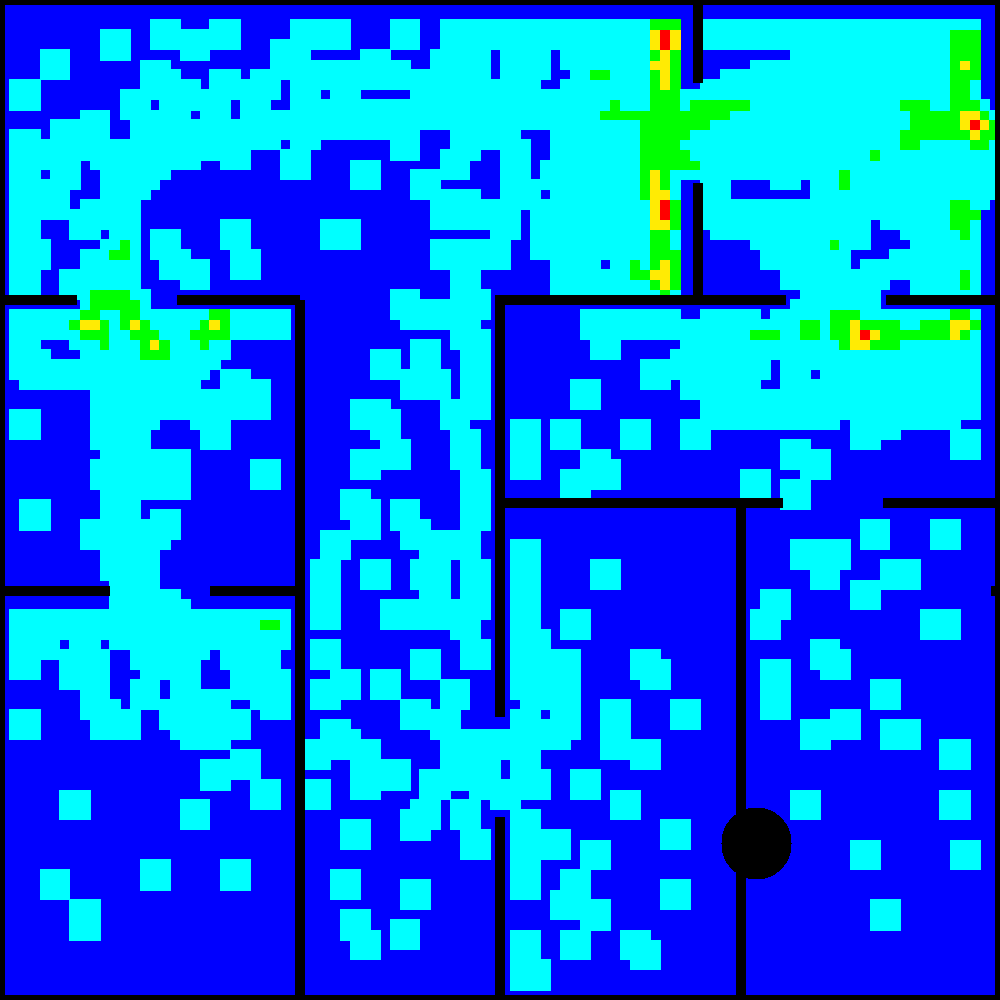
\includegraphics[width=0.19\textwidth]{images/Hypothesis2/Iter6-ID-17-t_8_151.png} \\
	Time=16.4175 & Time=13.695 & Time=11.1705 & Time=9.669 & Time=8.151
\end{tabular}
  \caption{\label{fig:codesign-incremental-improvement}Current best player's heatmap with  evacuation time for the crowd configuration LoS=F,LoA=High,LoH=Low in level 1}
  \begin{tabular}{c c c }
	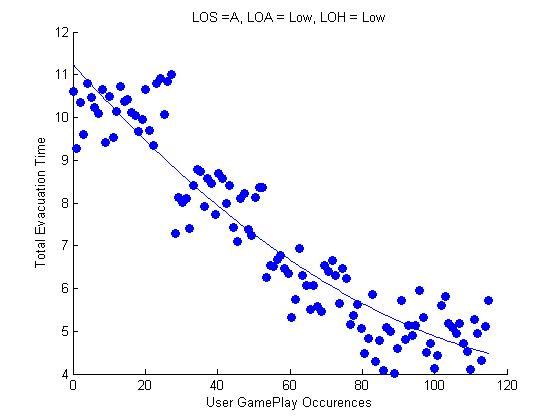
\includegraphics[width=0.31\textwidth]{images/Hypothesis2Graphs/LOS_A_LOA_Low_LOH_Low.jpg} &  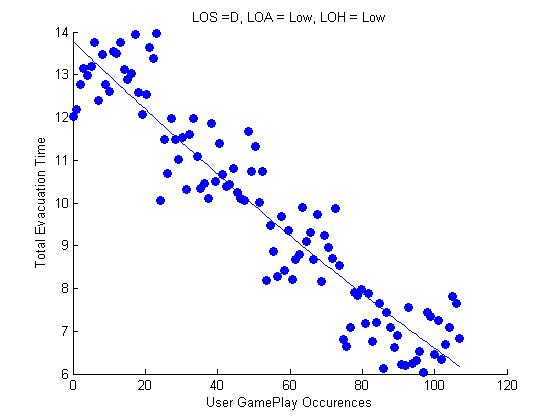
\includegraphics[width=0.31\textwidth]{images/Hypothesis2Graphs/LOS_D_LOA_Low_LOH_Low.jpg} &  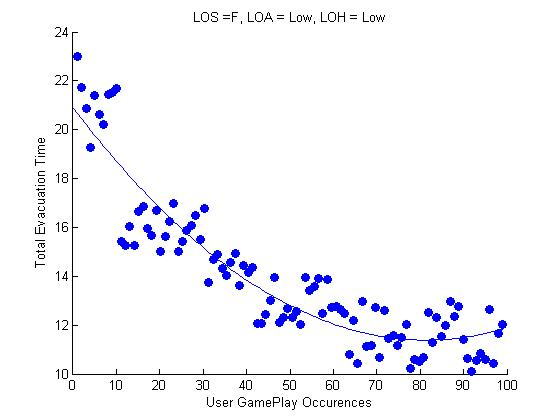
\includegraphics[width=0.31\textwidth]{images/Hypothesis2Graphs/LOS_F_LOA_Low_LOH_Low.jpg} \\
	LOS=A,LOA=Low,LOH=Low & LOS=D,LOA=Low,LOH=Low & LOS=F,LOA=Low,LOH=Low
\end{tabular}
  \caption{\label{fig:codesign-heatmap-changes}the Graphs of Evacuation Times for different User Gameplays in order of occurrence for 3 different combinations of crowd configuration parameters}
\end{figure*}

\subsection{Results}
In order to evaluate our hypotheses, we hosted our game on our website and asked people to play the game. We collected data for different users and for different levels. Analysing and comparing the results, we observed the following.

After analyzing the evacuation times of each user iterations for each level and each combination of crowd configurations, we have found a gradually decreasing curve of evacuation time in 73.33\% of total 60 user cases. In Figure~\ref{fig:single-player-iterative-improvement} we demonstrate a single case of iterative improvement of a design by a player using the crowd configuration Los=crowd density of 1.09-2.17, LoA=High, LoH=Low.To prove that we used the following method.

For each user we have calculated the following and plotted.
    \begin{equation}
\sum_{i=1}^{n_{A}-1} I(i+1,i)
 \end{equation}
    
    where, $n_{A}$ is the total number of iterations by an user A and
    
    \begin{equation*}
I(i+1,i) = \begin{cases}
1 &\text{$E_{i+1}$ - $E_{i}$ < 0.1}\  \\  -1 &\text{$E_{i+1}$-$E_{i}$ $\geq$ 0.1}
\end{cases}
\end{equation*}
where, $E_{i}$ is the evacuation time of user A's $i^{th}$ iteration. The threshold of difference in evacuation time between two consecutive iterations for a positive case is 0.1. We have then plotted the summation values from equation (2) for each user shown in histogram ~\ref{fig:histogram-of- positive-use-cases}. The bars beyond the 0, represents number of positive cases and the rest are number negative cases.

\begin{figure}
\centering
	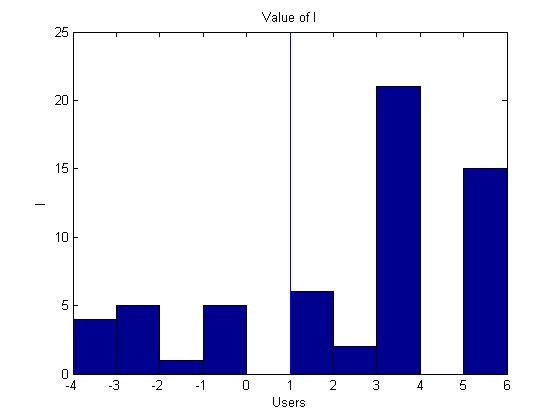
\includegraphics[width=0.3\textwidth]{images/ValueofI-Histogram.jpg} 
  \caption{\label{fig:histogram-of- positive-use-cases}The bars represents number of user. The positive user cases are beyond 0}
\end{figure}


For the second hypothesis, it was found that the evacuation times of different players viewing the current best scorer's heat map, gradually decreased and converged towards optimality. The curve formed by these players is very similar to that of a fitness function in computational optimization strategies. Figure~\ref{fig:codesign-incremental-improvement} is an example of this curve in which several player's iteratively improved a design by using the current best player's analyses and environment layout information. The Figure~\ref{fig:codesign-heatmap-changes} shows the Graphs of Evacuation Times for different User Gameplays in order of occurrence for 3 different combinations of crowd configuration parameters. 



\subsection{System Usability Results}
We are using the System Usability Scale to calculate the System Usability Scale(SUS) score~\cite{JBrookeSUS}. We received feedback from 61 players and calculated the score depending upon their responses. Our average usability score is 78.69 out of a scale of 100. Hence, our usability is average but there is a lot of scope for improvement.








